\documentclass[tikz,crop]{standalone}
\usepackage{tikz}
\usepackage{pgfplots}

\pgfplotsset{every axis/.append style={
    axis x line=middle,    % put the x axis in the middle
    axis y line=middle,    % put the y axis in the middle
    axis line style={<->}, % arrows on the axis
    xlabel={$x$},          % default put x on x-axis
    ylabel={$y$},          % default put y on y-axis
    },
    cmhplot/.style={color=red,mark=none,line width=1pt,<->},
    soldot/.style={color=red,only marks,mark=*},
    holdot/.style={color=red,fill=white,only marks,mark=*},
}

\usetikzlibrary{positioning, shapes, calc, shapes, arrows, decorations}



\tikzset{
	sigmoid/.style={
		path picture= {
    		\begin{scope}[x=4pt,y=4pt]
    		      \draw plot[domain=-1:1] (\x,{sign(\x)});
			\end{scope}
    	}
	}	
}


\tikzstyle{outputNode}=[draw,fill=gray!50,circle,minimum size=20pt,inner sep=0pt,sigmoid]
\tikzstyle{inputNode}=[draw,circle,minimum size=20pt,inner sep=0pt]
\tikzstyle{stateTransition}=[-stealth, thick]

\begin{document}
    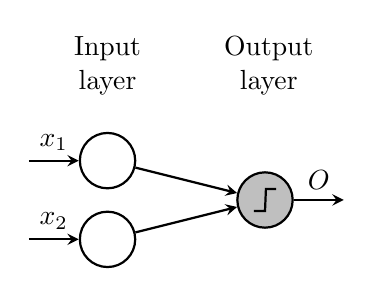
\begin{tikzpicture}
        \node[inputNode, thick] (i1) at (6, 1) {};
        \node[inputNode, thick] (i2) at (6, 0) {};




        \node[inputNode, thick, outputNode] (o1) at (8, 0.5) {};

        \draw[stateTransition] (5, 1) -- node[above] {$x_1$} (i1);
        \draw[stateTransition] (5, 0) -- node[above] {$x_2$} (i2);


        \draw[stateTransition] (i1) -- (o1);
        \draw[stateTransition] (i2) -- (o1);


        \node[above=1em of i1, align=center] (l1) {Input \\ layer};
        \node[right=2.3em of l1, align=center] (l3) {Output \\ layer};

        \draw[stateTransition] (o1) -- node[above] {$O$} (9, 0.5);


    \end{tikzpicture}
\end{document}